\documentclass[uplatex,dvipdfmx,12pt,a4j]{ujreport}

\usepackage{./sty/TitlePage}
\usepackage[dvipdfmx]{graphicx}
\usepackage[T1]{fontenc}
\usepackage{textcomp}
\usepackage[utf8]{inputenc}
\usepackage[uplatex]{otf}
\usepackage{listings,jlisting} % ソースコード読み込み用
\usepackage{color,url}
\usepackage{cite}
\usepackage{listings}
\usepackage{tikz}

\usetikzlibrary{positioning, shapes.geometric, arrows}

\lstset{
    basicstyle=\ttfamily\footnotesize,
    keywordstyle=\color{blue}\bfseries,
    stringstyle=\color{red},
    commentstyle=\color{green},
    frame=single,
    breaklines=true,
    numbers=left,
    numberstyle=\tiny,
    backgroundcolor=\color{white},
    tabsize=2,
    captionpos=b,
}

\tikzstyle{entity} = [rectangle, draw, minimum width=4cm, minimum height=1cm, text centered, node distance=2cm]
\tikzstyle{attribute} = [ellipse, draw, text centered, minimum width=3cm, font=\small]
\tikzstyle{relationship} = [diamond, draw, text centered, minimum width=2cm, font=\small]
\tikzstyle{line} = [draw, -latex]

\setlength {\oddsidemargin}{10.4mm}
\setlength {\evensidemargin}{10.4mm}
\baselineskip 17pt plus 1pt minus 1pt

\newcommand{\lw}[1]{\smash{\lower2.0ex \hbox{#1}}} % 表の中で位置を下にずらして書く

\makeatletter
\def\ngram{{\it n}-gram}
\def\@AppendixFirst{TRUE}
\def\appendix#1#2{%
  \def\true{TRUE}
  \ifx\@AppendixFirst\true
  \clearpage\pagenumbering{arabic}\setcounter{page}{1}%
  \setcounter{chapter}{0}%
  \def\@AppendixFirst{FALSE}
  \fi
  \addtocounter{chapter}{1}%
  \setcounter{figure}{0}%
  \renewcommand{\thefigure}{\Alph{chapter}.\@arabic\c@figure}%
  \renewcommand{\thetable}{\Alph{chapter}.\@arabic\c@table}%
  \def\addcontentsline##1##2##3{%
    \protected@write\@auxout
    {\let\label\@gobble \let\index\@gobble \let\glossary\@gobble\@temptokena{#1-\thepage}}%
    {\string\@writefile{##1}%
      {\protect\contentsline{##2}{##3}{\the\@temptokena}}}%
    }%
  \setcounter{section}{0}%
  \chapter*{付録 #1 #2}%
  \def\ps@jpl@in{%
    \def\@oddhead{\@empty}\def\@evenhead{\@empty}%
    \def\@oddfoot{\hfil{#1-\thepage}\hfil}%
    \def\@evenfoot{\hfil{#1-\thepage}\hfil}}%
  \pagestyle{jpl@in}%
  \setcounter{page}{1}%
  \addcontentsline{toc}{chapter}{付録 #1 #2}%
  \renewcommand{\thesection}{#1-\arabic{section}}}
\makeatother

\ronbun{~}


% ユーザー定義の色 (各自適宜変更)
\definecolor{OliveGreen}{cmyk}{0.64,0,0.95,0.40}
\definecolor{Pink}{rgb}{1,0.07,0.54}
\definecolor{CadetBlue}{cmyk}{0.62,0.57,0.23,0}
\definecolor{Brown}{cmyk}{0,0.81,1,0.60}
\definecolor{LightBrown}{rgb}{0.63,0.44,0}
\definecolor{Red}{rgb}{0.95, 0.35, 0.35}
\definecolor{Blue}{rgb}{0.20, 0.35, 0.85}


% ソースコード読み込み用 (各自適宜変更)
\lstset{
	language=C,
	basicstyle={\ttfamily\normalsize},
	identifierstyle={\small},
    % identifierstyle={\color{LightBrown}\small},
    commentstyle={\color{Brown}\normalsize\slshape},
	%keywordstyle={\normalsize\bfseries},
    keywordstyle={\color{Blue}\normalsize\bfseries},
    keywordstyle={[2]\color{Red}},        % Function
    keywordstyle={[3]\color{CadetBlue}},
	ndkeywordstyle={\color{LightBrown}\normalsize},
	stringstyle={\color{Pink}\normalsize},
    backgroundcolor={\color[gray]{.98}},
	frame={tb},
	breaklines=true,
	columns=[l]{fullflexible},
	numbers=left,
	xrightmargin=0zw,
	xleftmargin=3zw,
	% numberstyle={\normalsize},
    numberstyle={\ttfamily\small},
	stepnumber=1,
	numbersep=1zw,
	lineskip=-0.5ex,
	showstringspaces=false,
	tabsize=2,
	captionpos=b,
}

\shozoku{青山学院大学理工学部\\情報テクノロジー学科D\"{u}rst研究室}
\title{書類整理の自動化}
\author{嘉松 一汰}
\studentID{学籍番号:15820094}
\date{令和6年度}

\begin{document}

\maketitle
\pagenumbering{arabic}

\tableofcontents

\chapter{はじめに}
\label{ch:intro}

\quad

\section{研究背景}
\label{sec:research_bg}

日本企業の RPA (Robotics Process Automation~\cite{yasuhiro2017rpa})導入率は全体で38\%,中小企業では25\%となっており,非常に少ないことがわかる(図~\ref{fig:rpa_rate}).
また,大企業と中小企業の間に20\%以上の差があり,技術や規模による格差も見て取れる.これらの原因となっており要因として考えられることは,大きく分けて2つある.

1つ目は,RPAには専門領域と非専門領域が存在するということである.
専門領域はPC上の操作や,デジタルの領域における処理である.いっぽうで,紙媒体の処理等の,アナログの世界で実施される処理は非専門領域としている.
特に,手書きの文字や画像の認識を高い精度を保ちながら自動で処理することは,現代では非常に困難なことである.具体的には,縦書き文字横書き文字が混在していたり,旧字体や特殊文字等の組み合わせも考えられるため,例外的な処理までを自動でする必要があるからである~\cite{d-analyzer2019rpa}.

2つ目の原因は,紙媒体の業務を実施している企業のIT知識の乏しさにある.詳しくは次のセクションで説明する.このような現状を踏まえて,次章からは,OCR技術を使用したアプローチを提案する.

また,RPA の定義についても,明確には定まっていない部分が多い.自動化という概念自体に対して RPA という言葉を適用するとしたら,工場で食品の生産や梱包をするロボットも,我々の家で活躍するお掃除ロボットも,PC 上のボタン一つで複数の処理をするシステムも全て RPA と呼ぶことができる.
そのため,本研究では,RPA という言葉の意味を広義的に捉え,RPA の非専門領域で実施される処理を,他の様々な技術を用いて克服することを目標とする.
より詳細な技術については第\ref{ch:rt}章で述べるが,OCR や 字句解析の技術を使用し,紙媒体に対する処理を不自由なく自動化し,Ruby on Rails を使用したシステムとしての運用をして,我々の周りに多くある Web アプリケーションと同様に利用できるようにすることで,
IT に関する知識が乏しい企業でも,安全かつ快適に自動化の恩恵を受けることを目指す.

\clearpage
\begin{figure}[htbp]
\centering
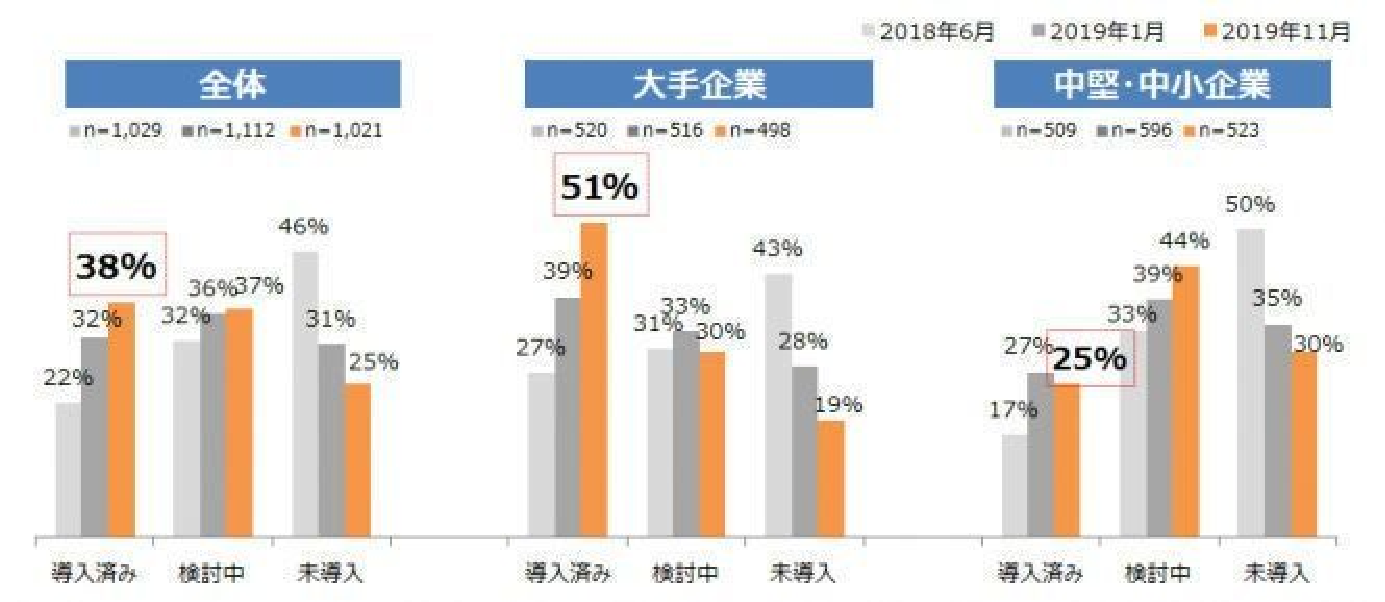
\includegraphics[scale = 0.6]{img/rpa_rate.pdf}
\caption{企業のRPA導入率}
\label{fig:rpa_rate}
\end{figure}%

\section{研究目的}
\label{sec:research_purpose}

本研究の目的は,IT 知識が乏しく,紙媒体の業務を実施している企業を中心に,RPA を使用して紙媒体の処理を自動で実施するシステムを作成することである.
具体的には,紙媒体の処理を OCR (Optical Character Recognition) 技術を用いてデジタルデータに変換し,さらに文字認識結果を用いた自動分類・ラベリングによって,手作業の削減と業務効率の向上を目指す.

日本で働く人事 ・ 総務担当者に,「紙媒体中心の業務で不便を感じたことがあるか?」とアンケートを取ったところ,61\%が不便を感じたことがあると回答した(図~\ref{fig:paper_media_survey}).
上記の理由として,システム障害への恐怖感や,IT知識の乏しさが挙げられる.多くの企業がデジタル化に対する適応を進めている中,依然として紙媒体を中心とした業務フローに頼らざるを得ない状況がある.
これにより,文書の管理や検索に時間がかかるだけでなく,人的ミスや紛失のリスクも存在する.

また,既存の RPA ソリューションでは紙媒体の取り扱いが難しく,専用の高価な機器が必要となる場合がある.
本研究では,これらの課題を克服し,誰でも簡単に使用できるシステムを設計・実装する.紙ベースの情報管理を効率化し,日常業務で活用できるようにする.

また,電子帳簿保存法の改正により~\cite{ito2023},企業は税務関連の書類や請求書などを電子データとして保存することが法的に求められるようになった.
この法律が施行されたことで,企業に対してある程度のデジタル化が義務付けられたことになる.本研究のシステムを導入することで,電子帳簿保存法に適合したデータ管理の効率化が期待できる.
これにより,企業のコンプライアンス遵守を支援し,業務負担の削減を目指す.

さらに,システムを Web アプリケーションとして提供し,スマートフォンやタブレットからも簡単にアクセス可能な形にすることで,
利便性向上を目指す.このような RPA ソリューションを普及させることにより,デジタル化が遅れている分野でも手軽に導入できる環境を提供し,業務の自動化を促進することを目指す.

\begin{figure}[htbp]
  \vspace{1cm}
  \centering
  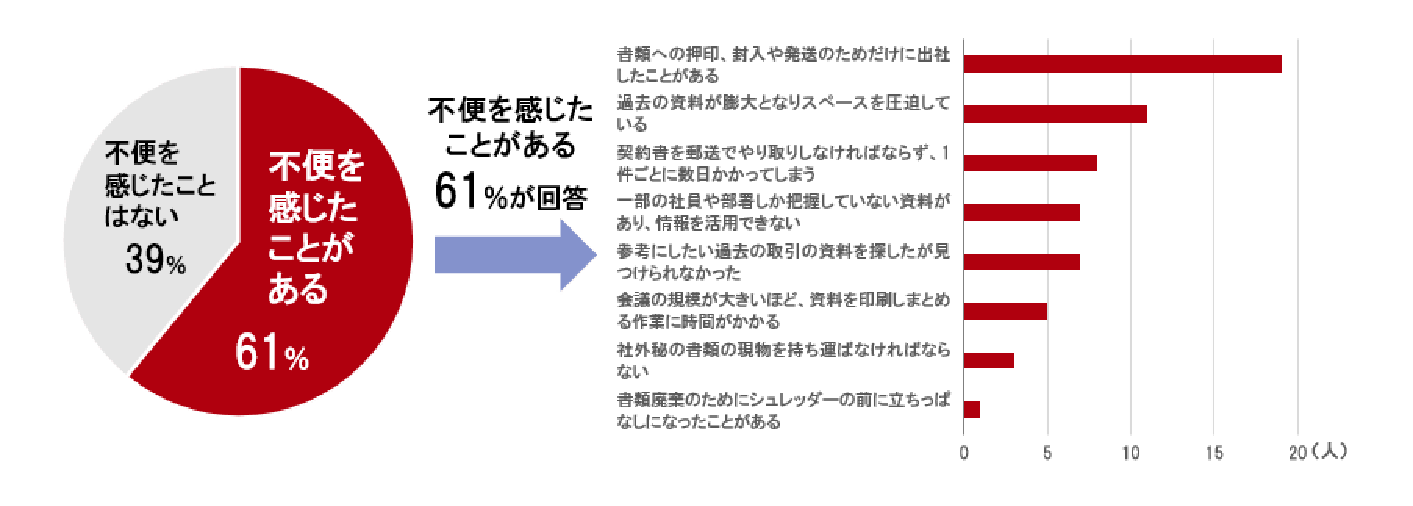
\includegraphics[scale = 0.6]{img/paper_media_survey.pdf}
  \caption{紙媒体中心業務に関するアンケート}
  \label{fig:paper_media_survey}
\end{figure}%

\section{論文の構成}
\label{sec_str}

本論文は7章構成になっている.第\ref{ch:intro}章では,本研究の背景や目的を述べた.第\ref{ch:rt}章では本研究で使用した基礎技術,関連技術を述べる.第\ref{ch:rw}章では,先行研究について説明し,本研究との差異を述べる.
本研究での実装手法を第\ref{ch:app}章で提案し,第\ref{ch:exp}章で実験と評価,第\ref{ch:eval}章で結果の考察を述べ,第\ref{ch:con}章でに本研究の総括をする.

\chapter{関連研究}
\label{ch:rw}

\quad

\section{RPA に関する研究}
\label{sec:rpa}

\subsection{RPA の歴史}
\label{subsec:rpa_history}

Madakam ら~\cite{Madakam2019}は,RPA の技術的発展とその適用範囲について調査している.RPA がどのように進化してきたか,また,どのような業務プロセスに適用されてきたかについて概観している.
RPA は,当初,単純な定型業務の自動化を目的として開発されたが,近年では AI (人工知能)や機械学習との統合が進み,より高度な業務への適用が可能になっている.
また,金融,ヘルスケア,製造業,行政機関など,さまざまな業界で RPA が活用されていることが示されている.

特に,RPA の適用事例として,人事業務,経理処理,請求書管理,データ移行などのバックオフィス業務における導入効果を詳細に分析している.
これらの業務は,本研究で開発するシステムの適用対象とも重なるため,本研究の有用性を裏付ける重要な知見となる.

\subsection{RPA の将来と可能性}
\label{subsec:rpa_future}

Lee ら~\cite{lee2023}は,RPA が雇用に与える影響について詳細に論じている.彼らの研究では,RPA が企業の業務効率化やコスト削減に寄与する一方で,人間の雇用に対する影響についても議論されている.
具体的には,RPA の導入が進むことで,反復的なルーチンタスクを自動化し,生産性の向上やミスの削減,24時間365日の稼働といったメリットをもたらすと述べられている.
しかしながら,RPA の普及によって,一部の業務が自動化されることで雇用の削減につながる可能性も指摘されている.

また,RPA が最も影響を与える業界や職種を特定し,企業の適応戦略についても分析している.特に,RPA の導入によってホワイトカラー業務のあり方が変化し,新たなスキル習得の必要性が高まっている点を強調している.
これらの知見は,RPA の導入に際して企業がどのような対策を講じるべきかを示唆するものであり,本研究の目的と関連性が高い.

\section{カテゴライズに関する先行研究}
\label{sec:categolize}

\subsection{機械学習を用いたカテゴライズ}
\label{subec:cate_study}

花房ら~\cite{hanabusa2015}は,プログラミング読解中の視線軌道を機械学習によりカテゴライズすることを試みた.従来,プログラミング技能の評価は主観的な評価や定性的な分析が中心であった.しかし,視線追跡データを用い,
教師あり学習を用いた学習モデルの1つである SVM (Support Vector Machine)を活用することにより,技能の異なる学習者(得意群・普通群・不得意群)の視線軌道パターンの定量的に分類した.
大学4年生24名を対象とし,C 言語のプログラムを提示しながら視線の動きを計測した.ヒートマップデータを簡略化し,視線パターンの特徴を抽出した.

任意のデータを定量的に分類し,精度を分析している点は,本研究と共通している.主観的評価に依存せず客観的な分析を実現している点は,機械学習によるカテゴライズの利点といえるだろう.
一方で,低難易度の問題では分類精度が低下したという結果から,解析結果の信頼性が,使用するデータセットに依存してしまう点は,カテゴライズの課題点だといえる.

\subsection{ドキュメントのカテゴライズ}
\label{subsec:cate_doc}

松田ら~\cite{matsuda1999}は,Web ページ(HTML 文書)を,HTML タグと,その要素の情報によってカテゴライズすることで,WWW 検索システムの拡張を試みた.従来の検索の仕組みは,
検索キーワードと全てのページを照合し,一致率の高い順番で表示する.しかし,あらかじめ,Web ページをいくつかのカテゴリに分類しておくことで,検索速度や,内容一致度の向上が見込まれる.

処理の具体的な流れを示す.カテゴライズの基準となる特徴記述ファイルを用意する.ファイル内には,タグと要素の組み合わせごとに,どのカテゴリに分類されるかの詳細な条件が記述されている.
読み込んだ HTML ファイルと特徴記述ファイルを比較し,文書のカテゴリを決定する.

文章に対して内容を解析し,カテゴライズするという点が本研究と共通している.特に解析方法について,Web ページ全体を複数の要素に分割し,各々に対して処理をした後に,
文書全体のカテゴリを判別するという流れは,本研究でも取り入れている.

\section{先行研究との比較}
\label{sec:rela}

\subsection{先行研究との類似点}
\label{subsec:same}

第~\ref{sec:categolize}節で示した2つの先行研究と同様に,特定の媒体に対してカテゴライズを実施しており,主観的な判断を排除しデータに基づく定量的な結果の分析を重視している.
特に松田らが実施した,カテゴライズに関する研究~\cite{matsuda1999}では,文書を要素ごとに分割し,それぞれのカテゴリを判別する手法を採用しているのに対し,本研究でも文書を単語レベルに分割し,各単語の定義を解析することで文書全体のカテゴリを決定するアプローチを採用している.

\subsection{先行研究との差異}
\label{subsec:diff}

一方で,これらの研究との大きな違いは,システムのコストパフォーマンスと拡張性である.花房らが実施した,視線誘導に関する研究~\cite{hanabusa2015}では,機械学習モデルを使用しているが,
このような高い精度を担保するモデルを1つの処理ごとに使用すると,時間的,金銭的にも高コストになってしまう.本研究では,そのような機械学習モデルは使用しておらず.少ないリソースで構築可能なシステムになっている.
さらに,拡張性に関しても,機械学習モデルを使用している場合はそのモデルにある程度依存した結果しか得られないが,本研究ではカテゴライズの条件を自由にカスタマイズできるため,各々の企業に最適なシステムを追求することができる.

また,松田らが実施した,文書タイプのカテゴライズに関する研究~\cite{matsuda1999}では,自身でカテゴライズの基準となるファイルを作成する必要があり.カテゴリが増えるたびに判別条件を考える必要がある.本研究では,単語の定義からカテゴライズするため,
カテゴリに該当する単語を容易に取得することができ,システムの構築や拡張段階において,コストを低く抑えることができる.

\chapter{提案手法}
\label{ch:app}
\quad

本研究で活用する手法,それに対するアプローチをはじめ,テーブルの構造や内容などのシステム設計を示す.
また,WordNet データベースとの連携方法に加えて,ドキュメントをどのようにカテゴライズするかを具体的に示す.

\section{システム設計}
\label{sec:app_design}
本研究のシステムのバックエンドに当たる部分を具体的に示す.
\subsection{データベース設計}
\label{subsec:table}

本研究で使用するテーブルには3種類ある.図 4.1に,これらを表す ER 図を示す.

\paragraph{Word テーブル}
Wordnet データベースの単語が格納されており,主キーである整数型の wordid カラム,言語を表す文字列型の lang カラム,単語名を表す文字列型の lemma カラムによって形成されている.

\paragraph{Synset テーブル}
WordNet データベースに含まれる単語の定義が格納されており,主キーである文字列型の synset カラム 定義名を表す name カラムによって形成されている.

\paragraph{Sense テーブル}
前述した2つのテーブルの中間テーブルであり,Word テーブルとの外部キーである wordid カラム,Synset テーブルとの外部キーである synset カラム,言語を表す文字列型の lang カラムによって形成されている.

\clearpage

\begin{figure}[h]
    \label{fig:er_diagram}
    \centering
    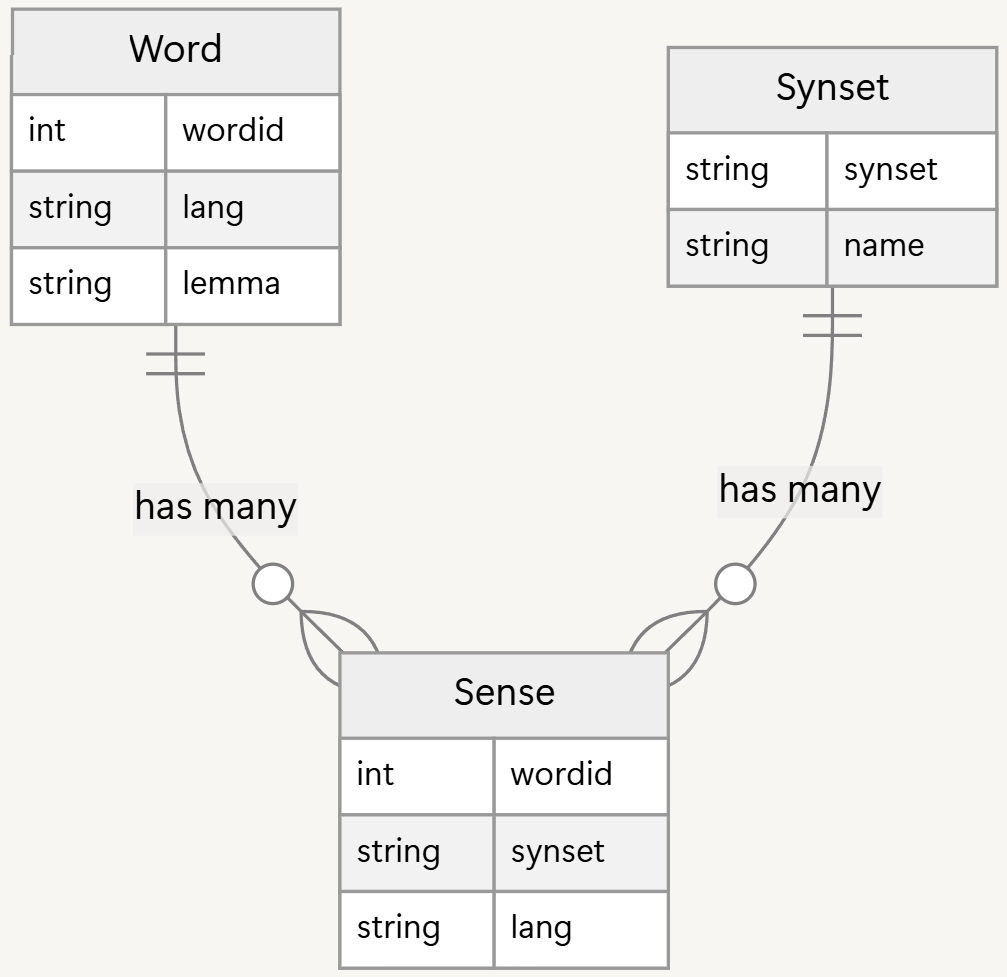
\includegraphics[scale = 0.4]{img/er_diagram.png}
    \caption{データベースの ER 図}
  \end{figure}

\subsection{モデル設計}
\label{subsec:model}

Ruby on Rails にはモデルという概念があり,データベースの内容をモデルとして定義することで,CRUD 処理を始めとしたバックエンドでのデータベースのやり取りを効率的にすることができる.
本研究では第~\ref{subsec:table}節で示したテーブルをモデルとして定義し,整合性等のデータベースレベルの具体的なプロパティを設定する.

\paragraph{Word モデル}
単語に関する情報が格納されている.Sense モデルと一対多の関係で,複数のSense モデルへのリレーションを持っており,Sense モデルを経由して,Synset モデルへのリレーションを辿ることで,単語からその定義を取得する.
場合に応じて適切な言語のレコードを活用するため,言語での絞り込みをするスコープを持つ.

\paragraph{Synset モデル}
単語の定義に関する情報が格納されている.主キーは文字列型の synset カラムである.Sense モデルと一対多の関係で,複数の Word モデルへのリレーションを持っており,Sense モデルを経由して,Word モデルへのリレーションを辿ることで,特定の定義をもつ単語を取得する.
Wordモデルと同様に,言語での絞り込みをするスコープを持つ.

\paragraph{Sense モデル}
Sense モデルは,上記の2つのモデルそれぞれと一対多のリレーションを持っている.synset カラムと wordid カラムが格納されており,それらを外部キーとして使用している.カラムと2つのモデルの双方向に紐づける役割を担う.単語と定義間で実行される処理は,Sense モデルを経由する.

\section{提案する手法 ・ アプローチ}
\label{sec:app_method}

本研究での手法の流れを以下に示す.始めに,カテゴライズしたいドキュメントファイルをシステムにアップロードする.その後,ファイルに対して OCR 処理をして,内容の単語群を取得する.
OCR と親和性のある代表的なプログラミング言語として Python が挙げられるが,http リクエストによって言語を問わず簡単に利用できる点や,OCR 処理に対するオプションの豊富さから,Google Vision API を本研究で使用する.
その後,WornNetデータベースと連携し,単語ごとの定義を取得する. WordNet は日本語,英語双方に対応した対規模な語彙データベースであるため,言語の入り混じったドキュメントに対しても問題なく処理をすることができるため,対応可能な語彙の量と汎用性を加味し,本研究で使用する.
各々の定義を元に単語がどのカテゴリに属するかを判別し,単語ごとにラベリングをする.ラベリング結果から,最終的なドキュメントのカテゴリを決定する.なお,各々のカテゴリに関しては,WordNet の Synset モデルにカテゴリ名を入力し,単語群を取得する方法で用意している.


\subsection{ドキュメントファイルをアップロード}
\label{subsec:app_upload}

Web上で動くRuby on Railsのシステムに対して,カテゴライズしたいドキュメントのファイルをアップロードする.
ファイルのアップロード用のアップローダークラスを定義し,詳しいオプションの設定をする.
アップロードされた画像ファイルのインスタンスをサービスクラスに渡し,OCR 等の処理をする.
上記の処理の流れをソースコード4.1に示す.

\begin{lstlisting}[language=HTML, caption=フロントエンドの ERB]
    <%= form_with(model: @document, url: '/', method: :post,
        multipart: true) do |form| %>
        <div class="form">
            <%= form.file_field :document_file %>
        </div>
        <%= form.submit 'アップロード' %>
    <% end %>
\end{lstlisting}

\subsection{OCRによってドキュメントの内容を取得}
\label{subsec:app_ocr}

Google Vision API の OCR 機能を用いて,ドキュメントの内容を取得し,単語ごとに分割する.
本研究では,まず OCR を実行するために Google Vision API を活用し,外部サービスと連携するためのサービスクラスを設計する.
このサービスクラス内で,API リクエストの送信処理やレスポンスの解析処理を行う.

まず VisionOcrService クラスのインスタンスを初期化する際に,画像認識のための ImageAnnotator::Client インスタンスを生成し,OCR を行う画像のパスを取得する.
次に,指定された画像ファイルの内容をバイナリ形式で読み込み,Vision API にリクエストを送信する.
API のレスポンスは,テキスト認識結果を保持するオブジェクトとして返される.このオブジェクト内から,OCR 結果として取得した文字列データをプロパティから抽出し,
単語の配列として整形する.処理の最終段階では,API 通信時のエラー処理として,ネットワークエラーや API 側の制限に伴う例外処理を行い,適切なエラーメッセージをログに記録することで,システムの信頼性を向上させる.
詳細な処理の流れをソースコード4.2に示す.

\begin{lstlisting}[language=Ruby, caption=Ruby による OCR の実装]
    require "google/cloud/vision/v1"

    class VisionOcrService
        def initialize(image_path)
            @image_path = image_path
            @vision = Google::Cloud::Vision::V1::
            ImageAnnotator::Client.new
        end

        def detect_text
            image_content = File.binread(@image_path)
            response = @vision.text_detection(image: {content:
            image_content})

            response.resources.flat_map do |res|
            res.text_annotations.map(&:description)
        end

        rescue StandardError => e
            Rails.logger.error "Vision API Error: #{e.message}"
            []
        end
    end
\end{lstlisting}

\subsection{それぞれの単語の定義の取得}
\label{sebsec:app_synset}

OCR によって取得した単語に対し,WordNet のデータベースを用いて定義を取得する.まず OCR の結果を配列形式でインスタンス変数に格納し,その後,分析プロセスを開始する.

具体的には,まず単語リストに対して,WordNet の Word テーブルから該当するエントリを検索し,関連する定義情報を取得する.
定義情報が見つからない場合は,"カテゴリ無し" として処理する.これらの処理は,OCR 結果のすべての単語に対して適用される.
最終的に,Synset テーブルの一覧をもとに,文書のカテゴリを判定するためのデータが整えられる.詳細な処理の流れをソースコード4.3に示す.

\begin{lstlisting}[language=Ruby, caption=ActiveRecord による WordNet との連携]
    class AnalyzeController < ApplicationController
        before_action :set_words, only: [:analyze]

        def analyze
            @category_labels = Hash.new(0)

            @words.each do |word|
                analyze_word = Word.includes(:synsets).find_by(lemma:
                word)
            return showNoCategoryError if analyze_word.nil?

            result_words = analyze_word.synsets.pluck(:name)
            current_labels = label_category(result_words)

            current_labels.each do |category, count|
                @category_labels[category] += count
            end
        end
            @result_category = get_category(@category_labels)
        end

        private
        def set_words
            @words = @ocr_response
        end
    end
\end{lstlisting}

\subsection{単語ごとにカテゴライズ,ラベリング}
\label{sebsec:app_categolize}

取得した単語の定義を基に,文書を適切なカテゴリに分類するためのラベリングを行う.
カテゴライズ処理では,WordNet から取得した Synset 情報をもとに,どの単語がどのカテゴリに属するかを決定する.システムは,各 Synset を解析し,それがどのカテゴリに該当するかを判別する.
この過程では,単語リストとカテゴリのマッピングをハッシュ形式で保持し,各カテゴリのカウントを増加させることで,どのカテゴリが最も関連性が高いかを測定する.

具体的には,単語を一意の集合として扱い,カテゴリごとの Synset 情報を取得し,対応するカテゴリラベルの数をカウントする.
これにより,文書内の単語がどのカテゴリに属しているかを判別し,最終的な文書のカテゴリ決定へと繋げる.詳細な処理の流れをソースコード4.4に示す.

\begin{lstlisting}[language=Ruby, caption=カテゴリのラベリングメソッド]
    def label_category(words)
        words_set = words.to_set

        categories = Category.all
        words_with_synsets = Word.where(lemma:
        categories.pluck(:value)).includes(:synsets)

        synsets_by_category = words_with_synsets
            .each_with_object({}) do |word, hash|
            hash[word.lemma] = word.synsets.map(&:name)
        end

        categories.each_with_object({}) do |category,
        category_labels|
            synset_names = synsets_by_category[category.value] || []
            label_count = synset_names.count { |name| words_set
                .include?(name) }
            category_labels[category.value] = label_count
        end
    end
\end{lstlisting}

\subsection{ラベリング結果から文章のカテゴリを決定}
\label{subsec:app_classify}

ラベリングされた結果をもとに文書の最終的なカテゴリを決定する.すべての単語に対してカテゴリが割り当てられた後,カテゴリごとのラベルカウントを集計し,最も多く出現したカテゴリを文書の主要カテゴリとして選定する.

まず受け取ったラベルデータのハッシュを解析し,カウント数が最大のカテゴリを特定する.
この処理の際,カテゴリが全く見つからなかった場合には,エラーをスローし,適切なメッセージを表示することで,未分類の文書に対する処理を明確化する.
最終的に,識別されたカテゴリは,文書全体のカテゴリとして出力される.詳細な処理の流れをソースコード4.5に示す.

\begin{lstlisting}[language=Ruby, caption=文書のカテゴリを決定するメソッド]
    def get_category(labels)
        max_label = labels.max_by { |_, value| value }
        if max_label[1] == 0
            showNoCategoryError
        else
            return max_label[0]
        end
    end

    def showNoCategoryError
        return 'no category'
    end
\end{lstlisting}

\chapter{実験・評価}
\label{ch:exp}
\quad

実際の業務環境における多様な文書形式に対する本システムの有効性を評価するため,実験用のカテゴリとドキュメントを用意し,カテゴライズを実施した.結果から,タイトル,カテゴリごとにドキュメントが適切なカテゴリに分類されているかを評価した.

\section{実験で使用したカテゴリ・ドキュメント}
\label{subsec:resource}

本研究では,経理,人事,庶務,営業,エンジニアリングの5カテゴリを対象として実験を実施した.これらのカテゴリは,組織運営における主要な業務部門を網羅しており,
各カテゴリごとにそれぞれ固有の専門用語やドキュメントの構造・フォーマットが異なる.例えば経理は会計関連の数値や伝票,人事は採用や労務管理に関する記述や採用の書類,庶務は各種連絡事項や管理文書,営業は提案書や顧客情報,エンジニアリングは技術仕様や設計書などが主となる.
そのため,分類アルゴリズムの精度および汎用性を包括的に評価する上で十分なサンプル群であるといえる.

また,ドキュメントに関しては,各カテゴリに対してドキュメントをを10個ずつ用意した.具体的には,企業で実際に利用される形式に類似したドキュメントを用いることで,システムの実務適用性を担保した.
また,フォントや字体,縦書き・横書きといった文書構成のバリエーションが多くなるように選定し,分類アルゴリズムがこれらの要素に対して正常に動作するかどうかの評価を実施した.

\clearpage

\section{精度の分析}
\label{sec:exp_anal}

\subsection{タイトルごとの精度}
\label{subsec:title}

タイトルごとの実験結果を表5.1 ~ 5.5に示す.

\begin{table}[!htbp]
  \label{tab:doc_accounting}
  \setlength{\abovecaptionskip}{5pt}
  \setlength{\belowcaptionskip}{5pt}
  \caption{経理カテゴリの精度}
  \begin{center}
  \begin{tabular}{|l|c|l|}
    \hline
    \textbf{タイトル} & \textbf{結果} & \textbf{備考} \\ \hline
    会社経理統制と経理検査 & \textcolor{red}{成功} & 昔の字体が存在する \\ \hline
    工業経理規範 & \textcolor{red}{成功} & 字体は全て昔の書き方 \\ \hline
    戦時会社経理統制体制の展開 & \textcolor{red}{成功} & 縦書き2列構成 \\ \hline
    法人税法の損金経理要件について & \textcolor{red}{成功} & 減価償却等の専門的な情報 \\ \hline
    陸軍経理組織の変遷と内部監査制度 & \textcolor{red}{成功} & \\ \hline
    企業における ERP システム導入 & \textcolor{red}{成功} & \\ \hline
    アスピレーションの欠如と管理会計 & \textcolor{red}{成功} & \\ \hline
    中小企業の内部統制の進め方 & \textcolor{blue}{失敗} & 内部統制に関する専門的な情報 \\ \hline
    日本の中小企業の会計情報システム & \textcolor{blue}{失敗} & 情報システム関連の単語が混在 \\ \hline
    中小企業の経営情報収集 & \textcolor{red}{成功} & \\ \hline
  \end{tabular}
  \end{center}
\end{table}

\begin{table}[!htbp]
  \label{tab:doc_human}
  \caption{人事カテゴリの精度}
  \begin{center}
  \begin{tabular}{|l|c|l|}
    \hline
    \textbf{タイトル} & \textbf{結果} & \textbf{備考} \\ \hline
    トヨタウェイと人事管理・労使管理 & \textcolor{red}{成功} & 縦書き2列構成 \\ \hline
    公務員の人事異動と人材形成 & \textcolor{red}{成功} & 図や英語が混在 \\ \hline
    新・人事労務管理 & \textcolor{red}{成功} & フォントがゴシック体の太文字 \\ \hline
    人事労務管理 & \textcolor{red}{成功} & 縦書きと横書きが混在 \\ \hline
    戦略的パートナーとしての日本の人事部 & \textcolor{red}{成功} & 図や見出しが英語表記 \\ \hline
    人事制度に関する総合調査 & \textcolor{red}{成功} & \\ \hline
    中小企業の従業員満足度 & \textcolor{red}{成功} & \\ \hline
    中小企業の新卒採用行動 & \textcolor{red}{成功} & \\ \hline
    日本企業におけるタレントマネジメント & \textcolor{red}{成功} & \\ \hline
    中小企業の人材育成 & \textcolor{blue}{失敗} & 図やグラフを使用した細かい分析 \\ \hline
  \end{tabular}
  \end{center}
\end{table}

\clearpage

\begin{table}[!htbp]
  \label{tab:doc_operation}
  \caption{庶務カテゴリの精度}
  \begin{center}
  \begin{tabular}{|l|c|l|}
    \hline
    \textbf{タイトル} & \textbf{結果} & \textbf{備考} \\ \hline
    RPA が事務職に及ぼす影響に関する一考察 & \textcolor{red}{成功} & \\ \hline
    一般事務女性の職業生活意識に関する一考察 & \textcolor{red}{成功} & 見出しのみ英語表記 \\ \hline
    女性事務職に得る派遣労働者の活用 & \textcolor{red}{成功} & 縦書き2列構成のゴシック体 \\ \hline
    女性事務職のキャリア拡大と職場組織 & \textcolor{red}{成功} & \\ \hline
    女性事務職の賃金と就業行動 & \textcolor{red}{成功} & \\ \hline
    事務作業における RPA の進展 & \textcolor{blue}{失敗} & エンジニアリング領域の単語 \\ \hline
    事務職のストレス状況調査 & \textcolor{red}{成功} & \\ \hline
    女性事務職のキャリア形成 & \textcolor{red}{成功} & \\ \hline
    ミクロデータを用いた女性事務職 & \textcolor{red}{成功} & \\ \hline
    大学の事務業務と効率化 & \textcolor{blue}{失敗} & 情報システム関連の単語 \\ \hline
  \end{tabular}
  \end{center}
\end{table}

\begin{table}[!htbp]
  \label{tab:doc_sales}
  \caption{営業カテゴリの精度}
  \begin{center}
  \begin{tabular}{|l|c|l|}
    \hline
    \textbf{タイトル} & \textbf{結果} & \textbf{備考} \\ \hline
    CRM 主要成功要因 & \textcolor{red}{成功} & CRM 関連の専門的な情報 \\ \hline
    チームワーク型営業のパフォーマンス & \textcolor{red}{成功} &  \\ \hline
    デジタル化と顧客経験価値 & \textcolor{blue}{失敗} & DX 分野の内容が多い \\ \hline
    営業組織のスキル可視化 & \textcolor{red}{成功} & 新人研修で使用するスライド形式 \\ \hline
    改善思考の営業プロセス管理 & \textcolor{red}{成功} & 縦書き2列構成 \\ \hline
    企業における営業力と管理体制 & \textcolor{red}{成功} & \\ \hline
    企業の営業力向上のために & \textcolor{red}{成功} & \\ \hline
    中小企業の営業組織強化法 & \textcolor{red}{成功} & \\ \hline
    小企業実態基本調査 & \textcolor{red}{成功} & \\ \hline
    日本における「営業」と「販売」 & \textcolor{red}{成功} & 縦書き2列構成 \\ \hline
  \end{tabular}
  \end{center}
\end{table}

\clearpage

\begin{table}[!htbp]
  \label{tab:doc_engineer}
  \caption{エンジニアリングカテゴリの精度}
  \begin{center}
  \begin{tabular}{|l|c|l|}
    \hline
    \textbf{タイトル} & \textbf{結果} & \textbf{備考} \\ \hline
    アジャイル開発の成功度 & \textcolor{red}{成功} & 英語と日本語が混在 \\ \hline
    組織的なソフトウェアプロセス改善 & \textcolor{red}{成功} &  \\ \hline
    大規模組織のソフトウェアプロセス改善 & \textcolor{red}{成功} & 縦書き2列構成 \\ \hline
    中小企業のソフトウェア品質改善 & \textcolor{red}{成功} & スライド形式 \\ \hline
    中小企業の IT 活動 & \textcolor{red}{成功} & \\ \hline
    中小企業のアジャイル開発のすすめ & \textcolor{red}{成功} & \\ \hline
    プロジェクトに対するリスク分析 & \textcolor{red}{成功} & \\ \hline
    円滑なマネジメントの失敗要因 & \textcolor{red}{成功} & 縦書き2列構成 \\ \hline
    プロジェクトの失敗回避に向けた分析 & \textcolor{red}{成功} & \\ \hline
    日本企業のオープンソース・ソフトウェア & \textcolor{red}{成功} & 英語と日本語が混在 \\ \hline
  \end{tabular}
  \end{center}
\end{table}

表5.1 ~ 5.5に示したように,処理精度にはタイトルごとにばらつきが見られる.特に,内容の専門性が高い文書や,他の分野の情報を多く含んでいる文書では処理が失敗する傾向が確認された.一方で,縦書きや横書きが混在する文書,英語表記が一部含まれる文書,ゴシック体や太文字を用いた文書などにおいては,ほとんど問題なく処理が成功している.これは,現代の標準的なフォーマットに近い文書に対しては,OCR の処理が適切に機能することを示している.
また,縦書き2列構成や図表が含まれる場合も成功率は高く,特に人事,営業,エンジニアリング関連のタイトルにおいては安定した処理精度が見られた.これらの結果から,フォーマットや字体の違いが OCR の精度に与える影響が明確になった.

\subsection{カテゴリごとの精度}
\label{subsec:category}

続いて,文書をカテゴリに分類し,それぞれのカテゴリごとに処理精度を評価した結果を表5.6に示す.

\begin{table}[h]
  \begin{center}
  \begin{tabular}{|c|r|}
    \hline
    \textbf{カテゴリ} & \textbf{精度 (\%)} \\ \hline
    経理 & 80 \\ \hline
    人事 & 90 \\ \hline
    庶務 & 80 \\ \hline
    営業 & 90 \\ \hline
    エンジニアリング & 100 \\ \hline
  \end{tabular}
  \end{center}
  \caption{カテゴリごとの精度}
  \label{tab:category_accuracy}
\end{table}

表5.6に示したように,経理カテゴリにおける精度が他のカテゴリと比べて低いことが確認された.この主な要因としては,経理カテゴリの文書に特殊な専門用語が多く含まれている点が挙げられる.
一方で,エンジニアリングカテゴリにおいては,フォーマットが比較的一般的であり,他のカテゴリの内容が含まれていることが少ないため,100\%の精度を達成している.
さらに,精度が高いカテゴリにおいても,処理内容には軽微な誤解釈が存在する場合があるが,全体としてカテゴリごとの分類精度に影響を与えるような問題は確認されなかった.これにより,OCR 処理のカテゴリごとの安定性について評価することができる.
以上の結果から,タイトルごとの処理精度とカテゴリごとの精度において,それぞれの特性が確認された.本研究では,特定の条件下における処理の成功率を明らかにしたが,さらなる精度向上を目指すためには,特殊なフォーマットへの対応が課題として残る.これらの詳細な考察については次章で述べる.

\chapter{考察}
\label{ch:eval}

\quad

\section{ドキュメントごとの結果の解釈}
\label{sec:eval_docs}

第~\ref{ch:exp}で本研究で行った実験を紹介したが,本章ではその結果から,本研究で提示したシステムの優位点及び将来性や有用性について述べる.
まず,実験により明らかとなった本システムの優位点について述べる.それは,ドキュメントの形式に関わらず同様の処理結果を得ることができる点である.
文書には,縦書きや横書き及びそれらの複合など,内容の形式はジャンルによって多岐にわたる.それら全てに対応出来なければ,本システムの優位性は著しく低下してしまう.
しかし,さまざまな形式の文書を実験では用意したが,特に形式の差による精度の変化は見受けられなかった.そのため,本システムにおいては,文書をアップロードする前に形式を確認する等の校閲を行う必要がなく,
その点ではストレスなくシステムを運用することができると考えられる.本システムの将来性については,発展途上であるという結論になってしまうが,将来的にカテゴリが増え,解析の幅が広がることや,
WordNet データベースにアップデートが行われ,扱うことのできる語彙が増えていくことを考えると, IT 分野の発展に伴い,相対的にニーズが増えていくと考えられる.
本システムの有用性については,第~\ref{ch:intro}で大まかに述べたが,紙媒体中心の業務に不便を感じている人が現代に多くいるため,そのような状況を改善するという観点では,要件を満たすことができているといえるだろう.

\section{改善点}
\label{sec:eval_improve}
本システムの欠点について挙げられることは,旧字体など,現在使用されていない字体を用いた文書に関しては,精度が落ちてしまう点である.
具体的には, OCR 処理では不自由なく単語ごとに分けることができているが, WordNet データベースにその単語が存在しないため,単語のカテゴリが判別できないことが原因として挙げられる.
また,機械学習を活用して未知の字体を動的に解析する技術を導入することも検討されるべきである.しかし,あくまで本システムは現代のコミュニティを対象としており,旧字体が記入された文書を取り扱うことは極めて少ないため,エンドユーザー視点では大きな欠点ではないといえる.
この欠点を改善するためには,現状使用している WordNet データべースの他に,漢字字体規範史データセットのような旧字体を扱っているデータベースを使用し,判別可能な語彙を拡張することが必要である.
これらを中心とした複数のデータベースを1つの MVC アーキテクチャに統合することができれば,本システムの有用性や汎用性の向上につながると考えられる.
また,現状のシステムでは,日本語と英語を主な対象としており, WordNet データベースを利用してカテゴリの解析を行っている.しかし,グローバル化が進む現代社会では,多言語対応が求められる場面が増えている.
特に,アジア地域で広く使用されている中国語,韓国語に対応することで,システムの利用範囲をさらに拡大することが可能である.
これを実現するためには,各言語に特化した語彙データベースを統合し,多言語間でのカテゴリ解析を可能にするアルゴリズムの開発が必要である.

\chapter{おわりに}
\label{ch:con}

\quad

\section{研究のまとめ}
\label{sec:con_fin}

本研究で開発したシステムは,現在の業務フローにおける課題を解決し得る有効なツールであると結論付けられる.また,さらなる改良を通じて,専門分野や多言語対応,クラウドサービス化といった新たな領域への応用が期待される.
現代では,今後も IT 分野の著しい成長に遅れをとった企業を中心に,さまざまな業務的ニーズが発生すると考えられる.本研究では紙媒体中心業務をさらに細分化した,
ドキュメントのカテゴライズ分野に着目してシステムの作成をしたが,本システムのようなソリューションが生み出されることで,IT 社会の課題が解決されることを願っている.

\section{今後の展望}
\label{sec:con_future}

本システムを現実的な業務フローに組み込むには,ユーザーインターフェース(UI)の最適化も重要である.現状ではシステムのコア機能に重点を置いているが,操作の直感性やユーザーエクスペリエンスの向上が求められる.
例えば,解析結果を可視化するダッシュボードや,フィードバック機能を備えたインターフェースを実装することで,利用者の利便性を高めることが可能である.
処理の精度について,経理,人事,処務といったカテゴリにおいて,高い精度での解析が可能であることが確認された.本システムはさらに分野ごとに特化した最適化を施すことで,
専門分野への応用を推進できる,例えば医療分野や法律分野では特有の専門用語や文書構造が存在するため,分野別にカスタマイズされた解析アルゴリズムが必要である.
また,本システムをクラウドベースで提供することにより,複数のユーザーが同時に利用できる環境を構築し,スケーラビリティを確保することができる.また,APIを公開することで,他のアプリケーションやサービスとの統合を可能にし,システムの拡張性をさらに高めることも有効である.


\newpage
\addcontentsline{toc}{chapter}{参考文献}
\renewcommand{\bibname}{参考文献}
\bibliographystyle{jplain}
\bibliography{biblio}

\end{document}
